\newpage
\subsection{QuizziPedia::Front-End::ServiceWorker}


\begin{figure} [ht]
	\centering
	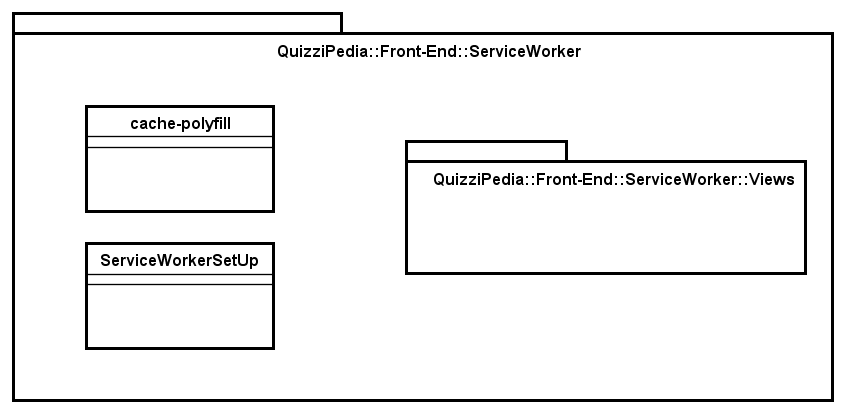
\includegraphics[scale=0.42]{UML/Package/QuizziPedia_Front-End_ServiceWorker.png}
	\caption{QuizziPedia::Front-End::ServiceWorker}
\end{figure} \FloatBarrier

\subsubsection{Informazioni generali}
\begin{itemize}
	\item \textbf{Descrizione}:	\textit{package\ped{G}} contenente le classi e i \textit{package\ped{G}} che definiscono la logica dell'applicazione offline;
	\item \textbf{Padre}: \texttt{Front-End};
	\item \textbf{Interazione con altri componenti}:
	\begin{itemize}
		\item \texttt{ServiceWorker::Views}: \textit{package\ped{G}} contenente le \textit{views\ped{G}} front-end dell'applicazione offline.
	\end{itemize} 
\end{itemize}
\subsubsection{Classi}

\paragraph[QuizziPedia::Front-End::ServiceWorker::cache-polyfill]{QuizziPedia::Front-End::ServiceWorker::cache-polyfill}
\begin{figure} [ht]
	\centering
	\includegraphics[scale=0.80]{UML/Classi/Front-End/QuizziPedia_Front-End_ServiceWorker_cache-polyfill.png}
	\caption{QuizziPedia::Front-End::ServiceWorker::cache-polyfill}
\end{figure} \FloatBarrier
\begin{itemize}
	\item \textbf{Descrizione}: ;
	\item \textbf{Utilizzo}: ;
	\item \textbf{Relazioni con altre classi}:
	\begin{itemize}
		\item \textbf{IN};
		\item \textbf{OUT}.
	\end{itemize}
	\item \textbf{Metodi}:
\end{itemize}


\paragraph[QuizziPedia::Front-End::ServiceWorker::ServiceWorkerSetUp]{QuizziPedia::Front-End::ServiceWorker::ServiceWorkerSetUp}
\begin{figure} [ht]
	\centering
	\includegraphics[scale=0.80]{UML/Classi/Front-End/QuizziPedia_Front-End_ServiceWorker_ServiceWorkerSetUp.png}
	\caption{QuizziPedia::Front-End::ServiceWorker::ServiceWorkerSetUp}
\end{figure} \FloatBarrier
\begin{itemize}
	\item \textbf{Descrizione}: ;
	\item \textbf{Utilizzo}: ;
	\item \textbf{Relazioni con altre classi}:
	\begin{itemize}
		\item \textbf{IN};
		\item \textbf{OUT}.
	\end{itemize}
	\item \textbf{Metodi}:
\end{itemize}


\newpage
\subsubsection[QuizziPedia::Front-End::ServiceWorker::Views]{QuizziPedia::Front-End::ServiceWorker::Views}
\begin{figure} [ht]
	\centering
	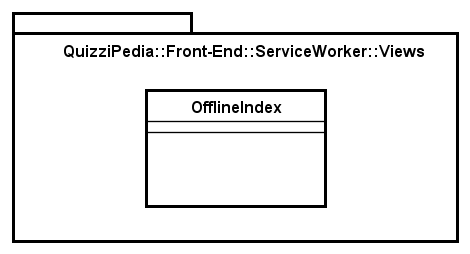
\includegraphics[scale=0.80]{UML/Package/QuizziPedia_Front-End_ServiceWorker_Views.png}
	\caption{QuizziPedia::Front-End::ServiceWorker::Views}
\end{figure} \FloatBarrier

\subsubsection{Informazioni generali}
\begin{itemize}
	\item \textbf{Descrizione}: package contenente le views front-end dell'applicazione offline;
	\item \textbf{Padre}: \texttt{ServiceWorker}.
\end{itemize}
\subsubsection{Classi}

\paragraph[QuizziPedia::Front-End::ServiceWorker::Views::OfflineIndex]{QuizziPedia::Front-End::ServiceWorker::Views::OfflineIndex}
\begin{figure} [ht]
	\centering
	\includegraphics[scale=0.80]{UML/Classi/Front-End/QuizziPedia_Front-End_ServiceWorker_Views_OfflineIndex.png}
	\caption{QuizziPedia::Front-End::ServiceWorker::Views::OfflineIndex}
\end{figure} \FloatBarrier
\begin{itemize}
	\item \textbf{Descrizione}: \textit{view\ped{G}} generale dell'applicazione offline;
	\item \textbf{Utilizzo}: contiene gli elementi che saranno presenti nella pagina dell'applicazione offline.
\end{itemize}




